\documentclass[a4paper,12pt]{article}
\usepackage[spanish]{babel} 
\usepackage{amsmath} 
\usepackage[colorlinks=true]{hyperref}
\usepackage{enumitem} 
\usepackage{graphicx}   
\usepackage[a4paper,top=3cm,bottom=3cm,left=3cm,right=3cm,marginparwidth=1.75cm]{geometry} 
\usepackage[]{subfigure}
\usepackage[]{multicol}

\graphicspath{ {./imag/Lab-Termo/Git/Documentos}} 
\title{Jaula de Faraday} 
\author{Noemi de la Peña, Benjamín Opazo, Martina Contreras \\ \\
 \textit{ Departamento de Física, Universidad de Concepción, Concepción, Chile. }}
  \date{} 

  



   %==================================================================================
\begin{document}
\maketitle 



%=============Resumen.
En este presente documento se expondra datos y concluciones 
obtenidas a traves de 3 diferentes experimentos.Relacionados con el campo electrico,
conductores y las ondas electro magneticas.



%========Introducción
\section*{Introdución}
    A medida que el saber del humano crece, tambien lo hace las preguntas.
    ¿Porque al frotar un globo sobre mi cabeza los pelos se levantan? o 
    ¿Por qué cae un rayo?
    Los antiguos griegos dieron incapie a el estudio de la ciencia que 
    lograria dar respuesta a las anteriores interrogantes, El electromagnetismo.
%==============Marco teorico
\section*{Marco teorico}
\begin{enumerate}
    \item electromagnetismo:
    \item Campos magneticos:
    \item Conductores:
    \item Jaula de faraday:
\end{enumerate}

%========Objetivos
%\section{Objetivos}
%\begin{itemize}
   
%\end{itemize}


%=========Marco Teórico
%\section{Marco Teórico}




%=========Materiales
\section*{Materiales}
\begin{multicols}{2}
\begin{itemize}
    \item celular
    \item papel de aluminio
    \item jabón
    \item agua
    \item globo
    \item bombilla
    \item bolsa ziploc
    \item audífonos
    \item colador de metal 
\end{itemize}
\end{multicols}


%%%%%%%%%%%%%%%%%%%%%%%%Procedimiento
\section*{Experimento 1}
\textit{Materiales: Papel de aluminio, celular.}
\begin{itemize}
    \item Primero, Debemos asegurarnos de que el celular pueda resivir llamadas de forma correcta.
    \item Segundo, ponemos el celular sobre el papel de aluminio.
    \item Tercero, desde otro móvil, llamamos al celular del esperimento para comprobar que funciona correctamente.
    \item Luego envolvemos el celular con el papel de aluminio.
    \item Finalmente volvemos a llamar, para notar el efecto que tiene el papel de alumio sobre el celular.
\end{itemize}
%Imagenes%
\begin{figure}[h]
    \begin{subfigure}
        \raggedright
        \includegraphics[width=4cm, height=5cm]{imag/Exp1_00.jpg}
        \end{subfigure}
    \begin{subfigure}
        \centering
        \includegraphics[width=4cm, height=5cm]{imag/Exp1_01.jpg}
    \end{subfigure}
    \begin{subfigure}
        \raggedleft
        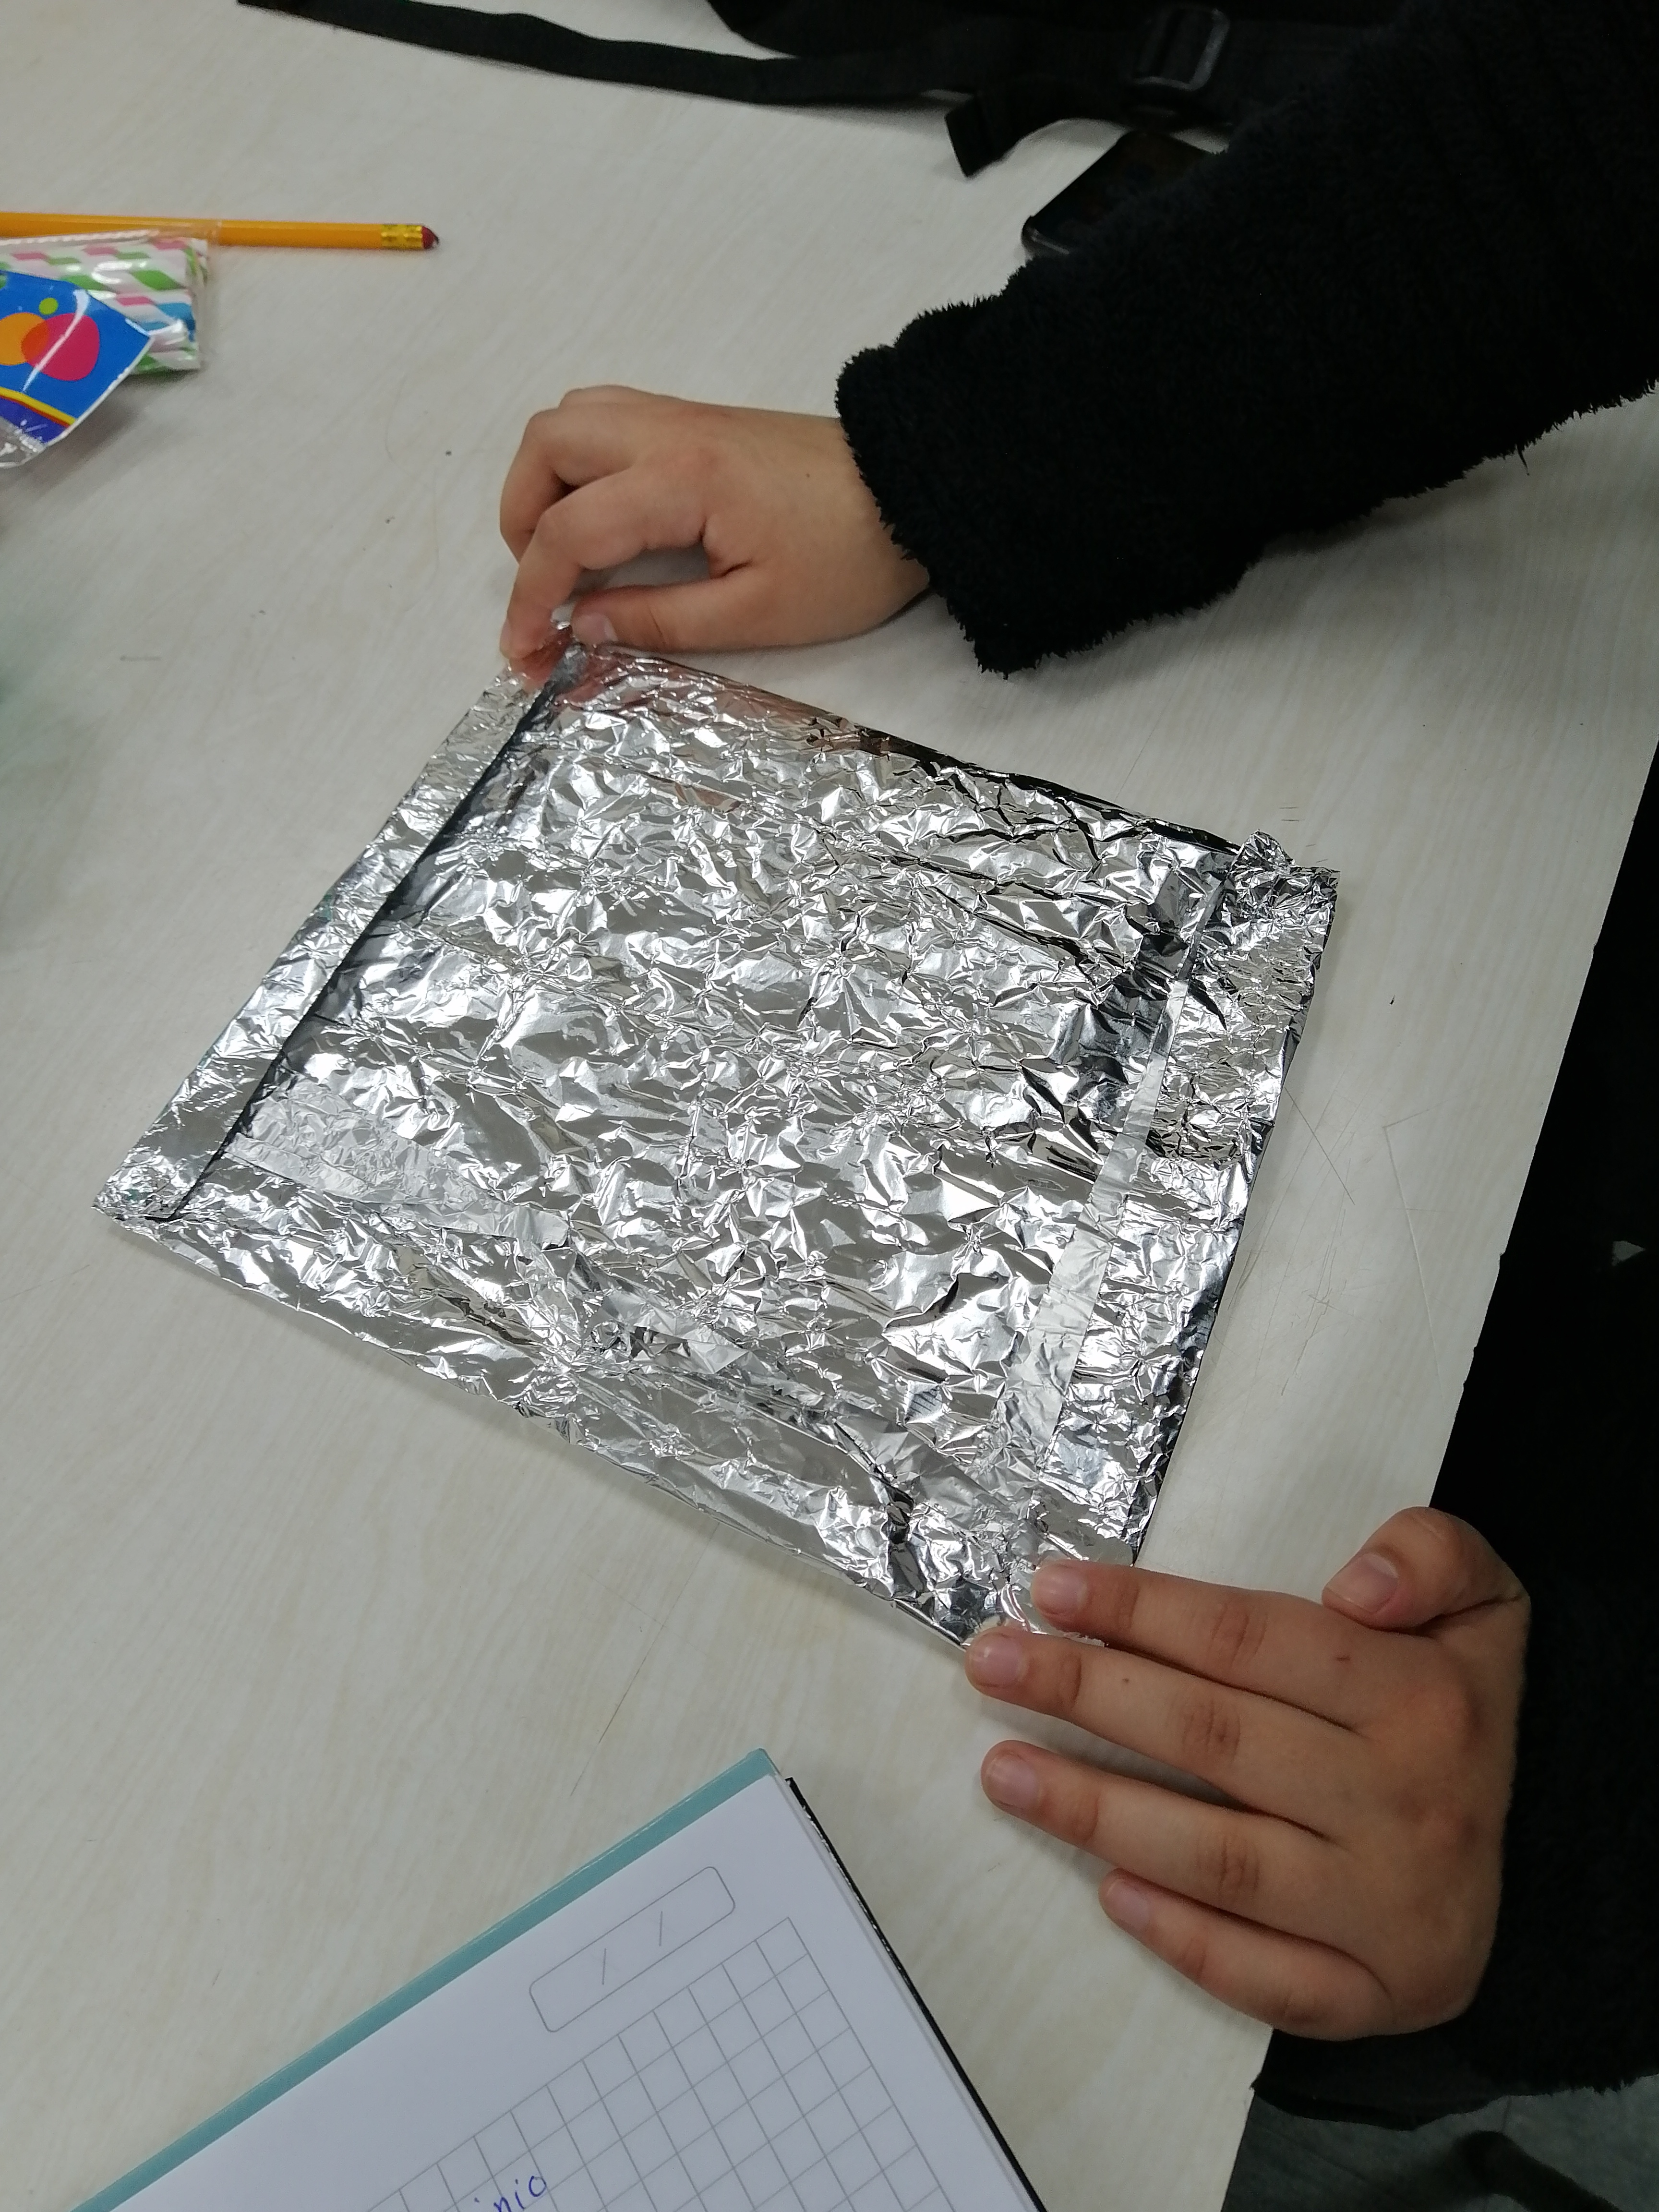
\includegraphics[width=4cm, height=5cm]{imag/Exp1_02.jpg}
    \end{subfigure}
\end{figure}
%%%%%%%%%%%%%%%%%%%%%%%%%%%%%%%%%%%%%%%%%%%%%%%%%%%%%%%%%%

\section*{Experimento 2}
\textit{Materiales: Jabón, agua, bombilla, globo, bolsa ziploc.}
\begin{itemize}
    \item Primero mezclamos el agua con el jabón.
    \item Segundo, sobre la bolsa ziploc, desparramamos un poco de la mezcla hecha anteriormente.
    \item Luego, con una bombilla hacemos una burbuja grande y acercamos el globo, ya inflado, para notar el efecto que tiene sobre la burbuja.
    \item Despues, volvemos hacer otra burbuja,pero en el interior de la burbuja inicial y repetimos el procedimiento hecho con el globo.
\end{itemize}

%Imagenes%
\begin{figure}[h]
    \begin{subfigure}
        \raggedright
        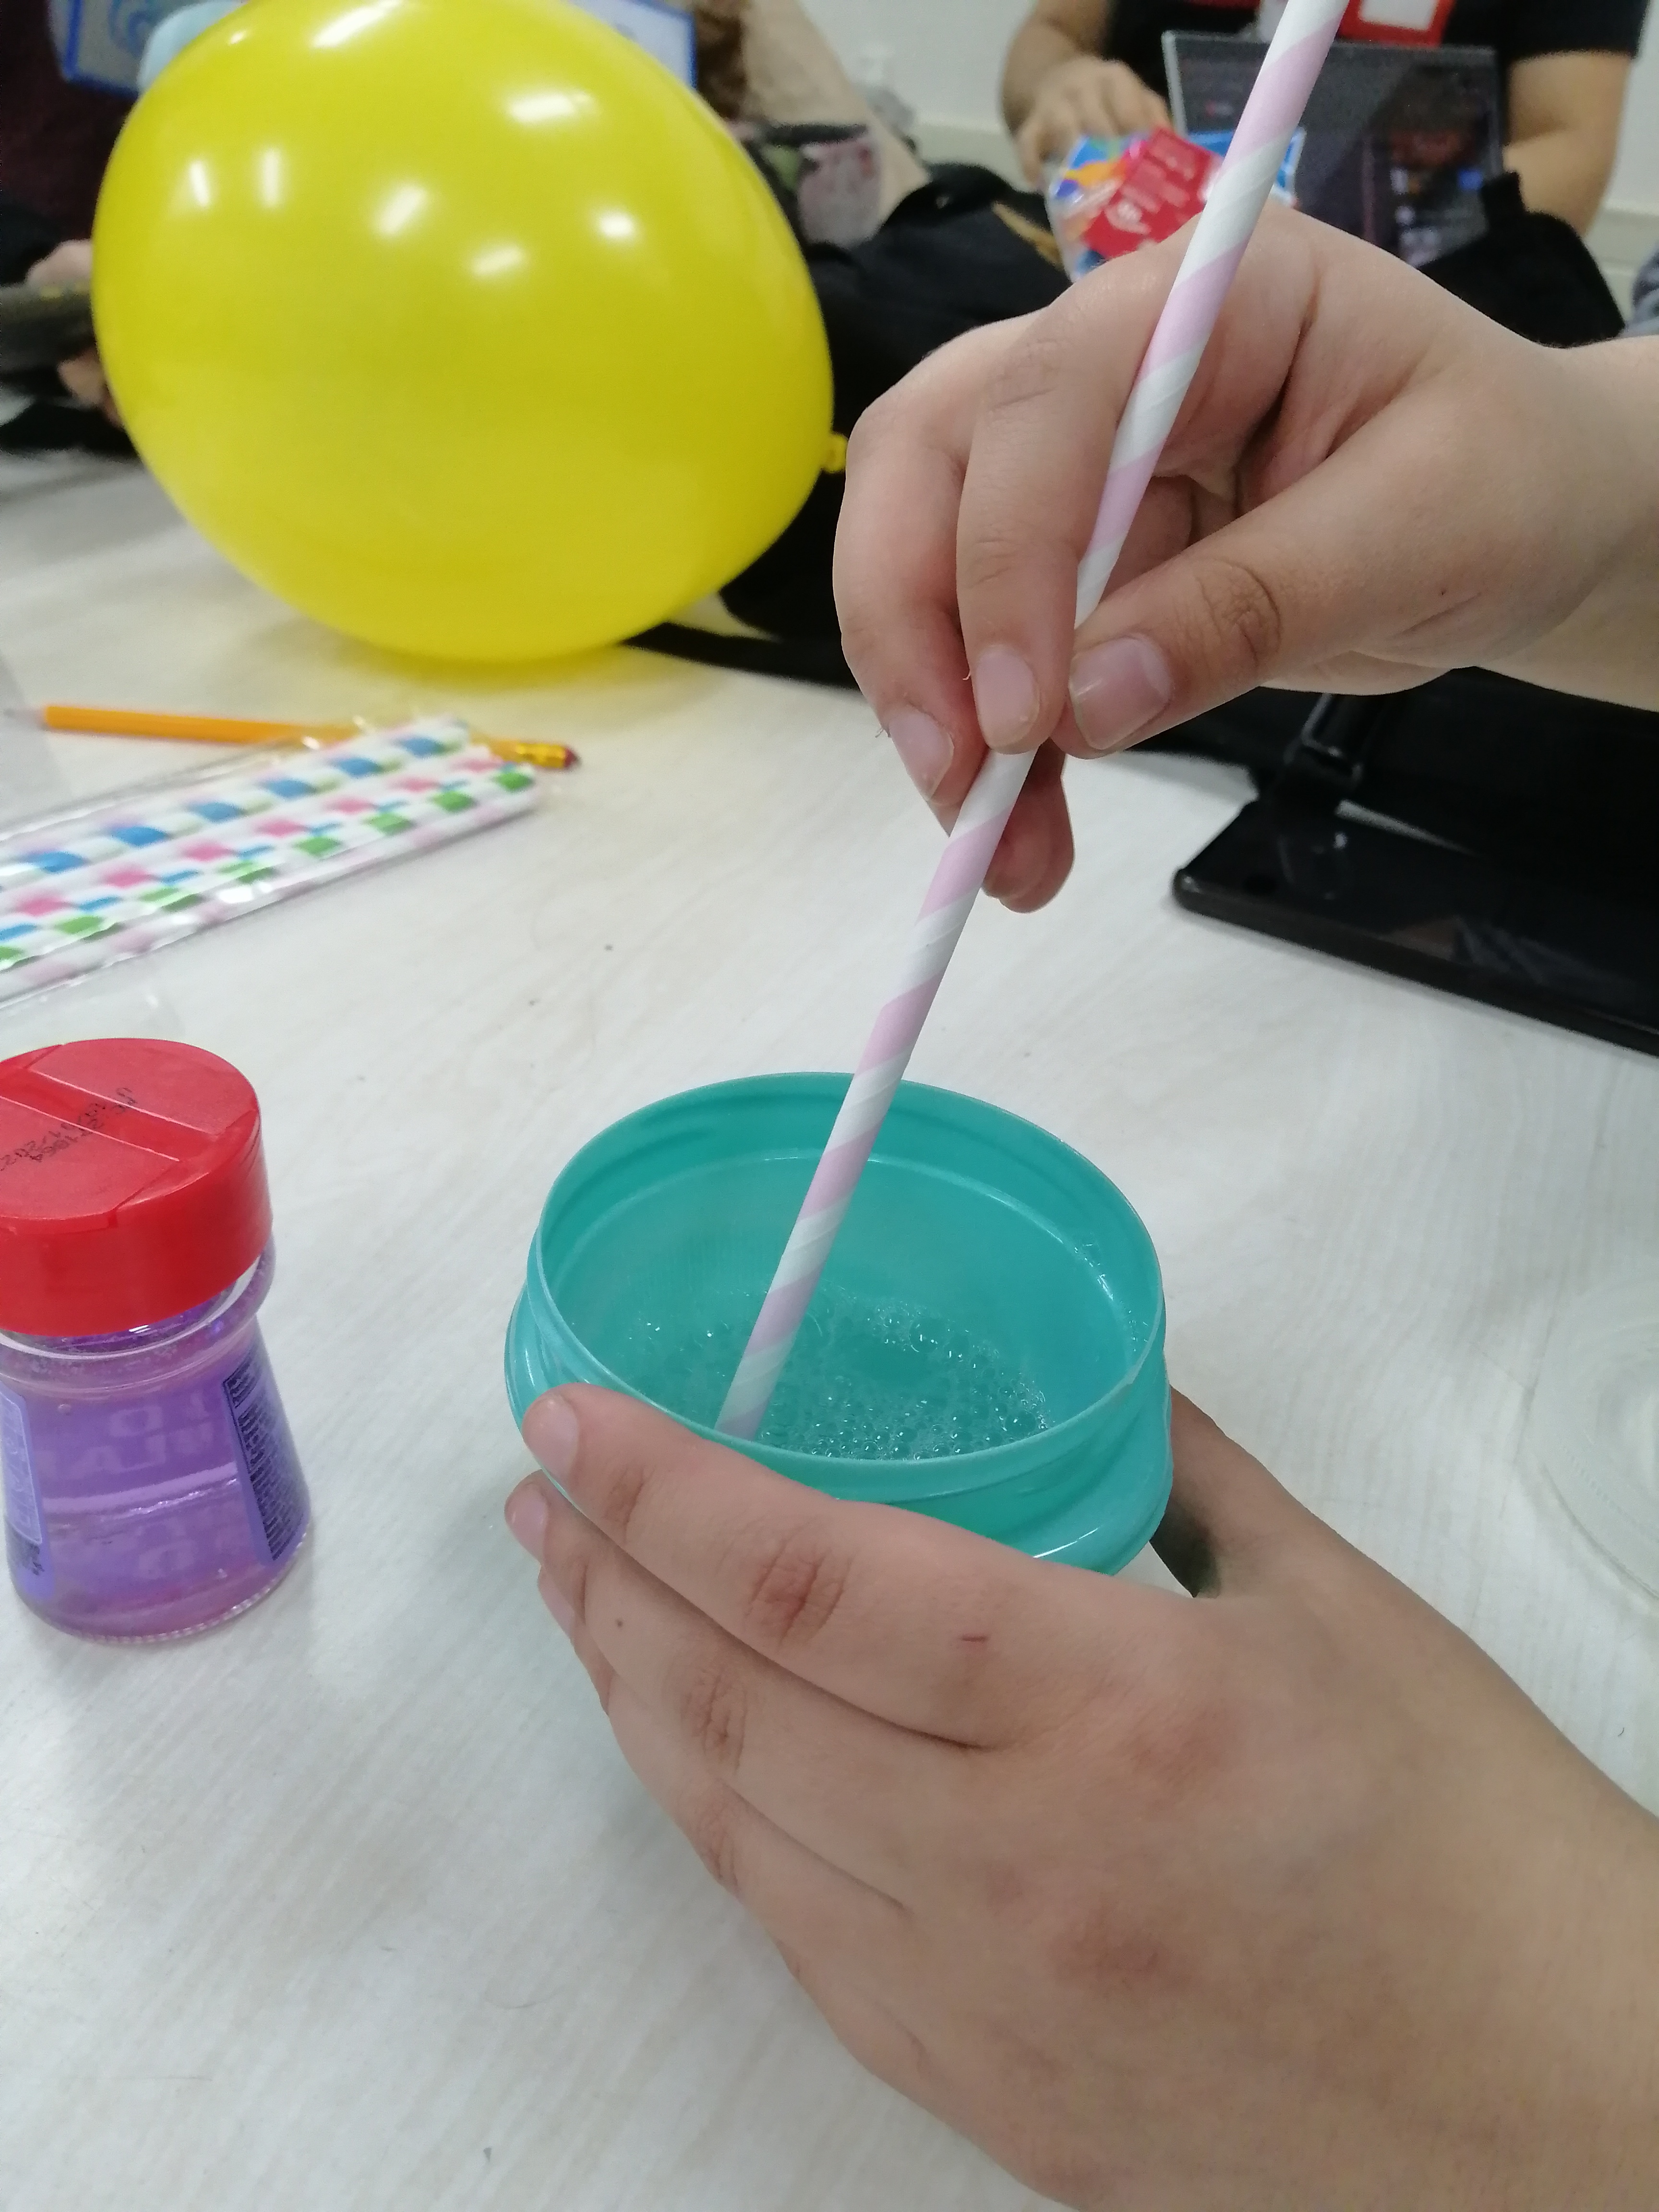
\includegraphics[width=4cm, height=5cm]{imag/Exp2_00.jpg}
    \end{subfigure}
    \begin{subfigure}
        \centering
        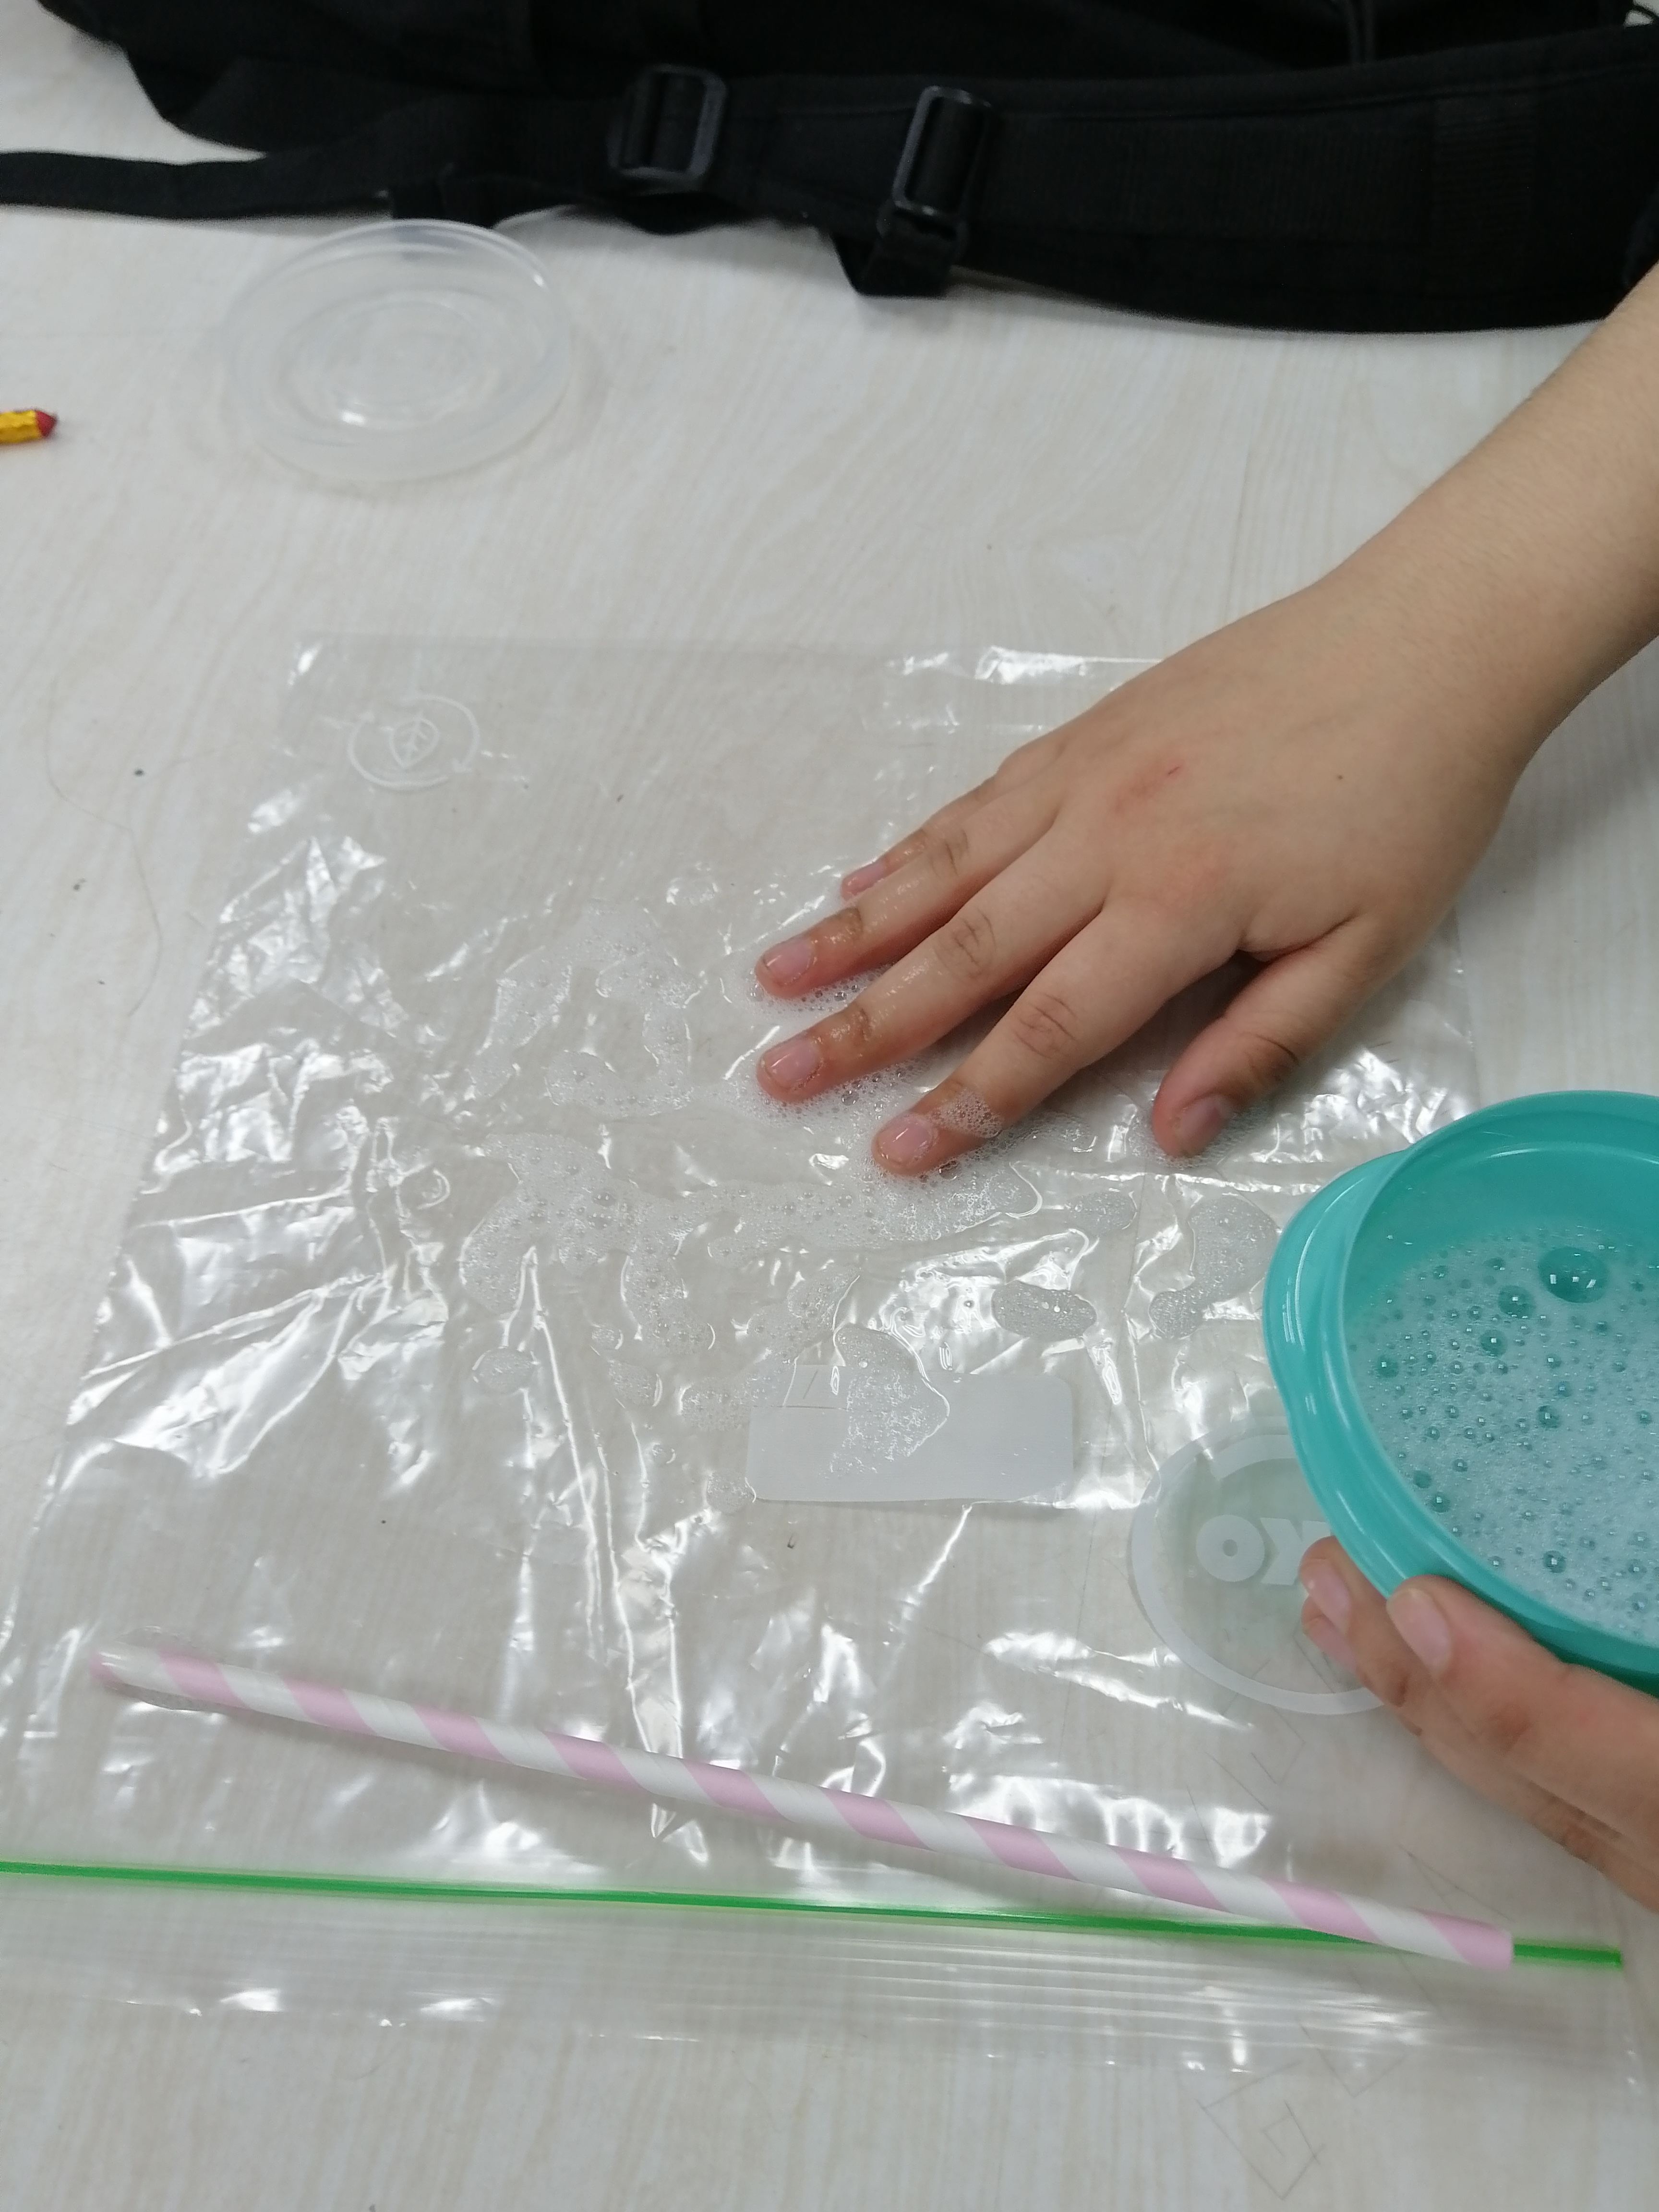
\includegraphics[width=4cm, height=5cm]{imag/Exp2_01.jpg}
    \end{subfigure}
    \begin{subfigure}
        \raggedleft
        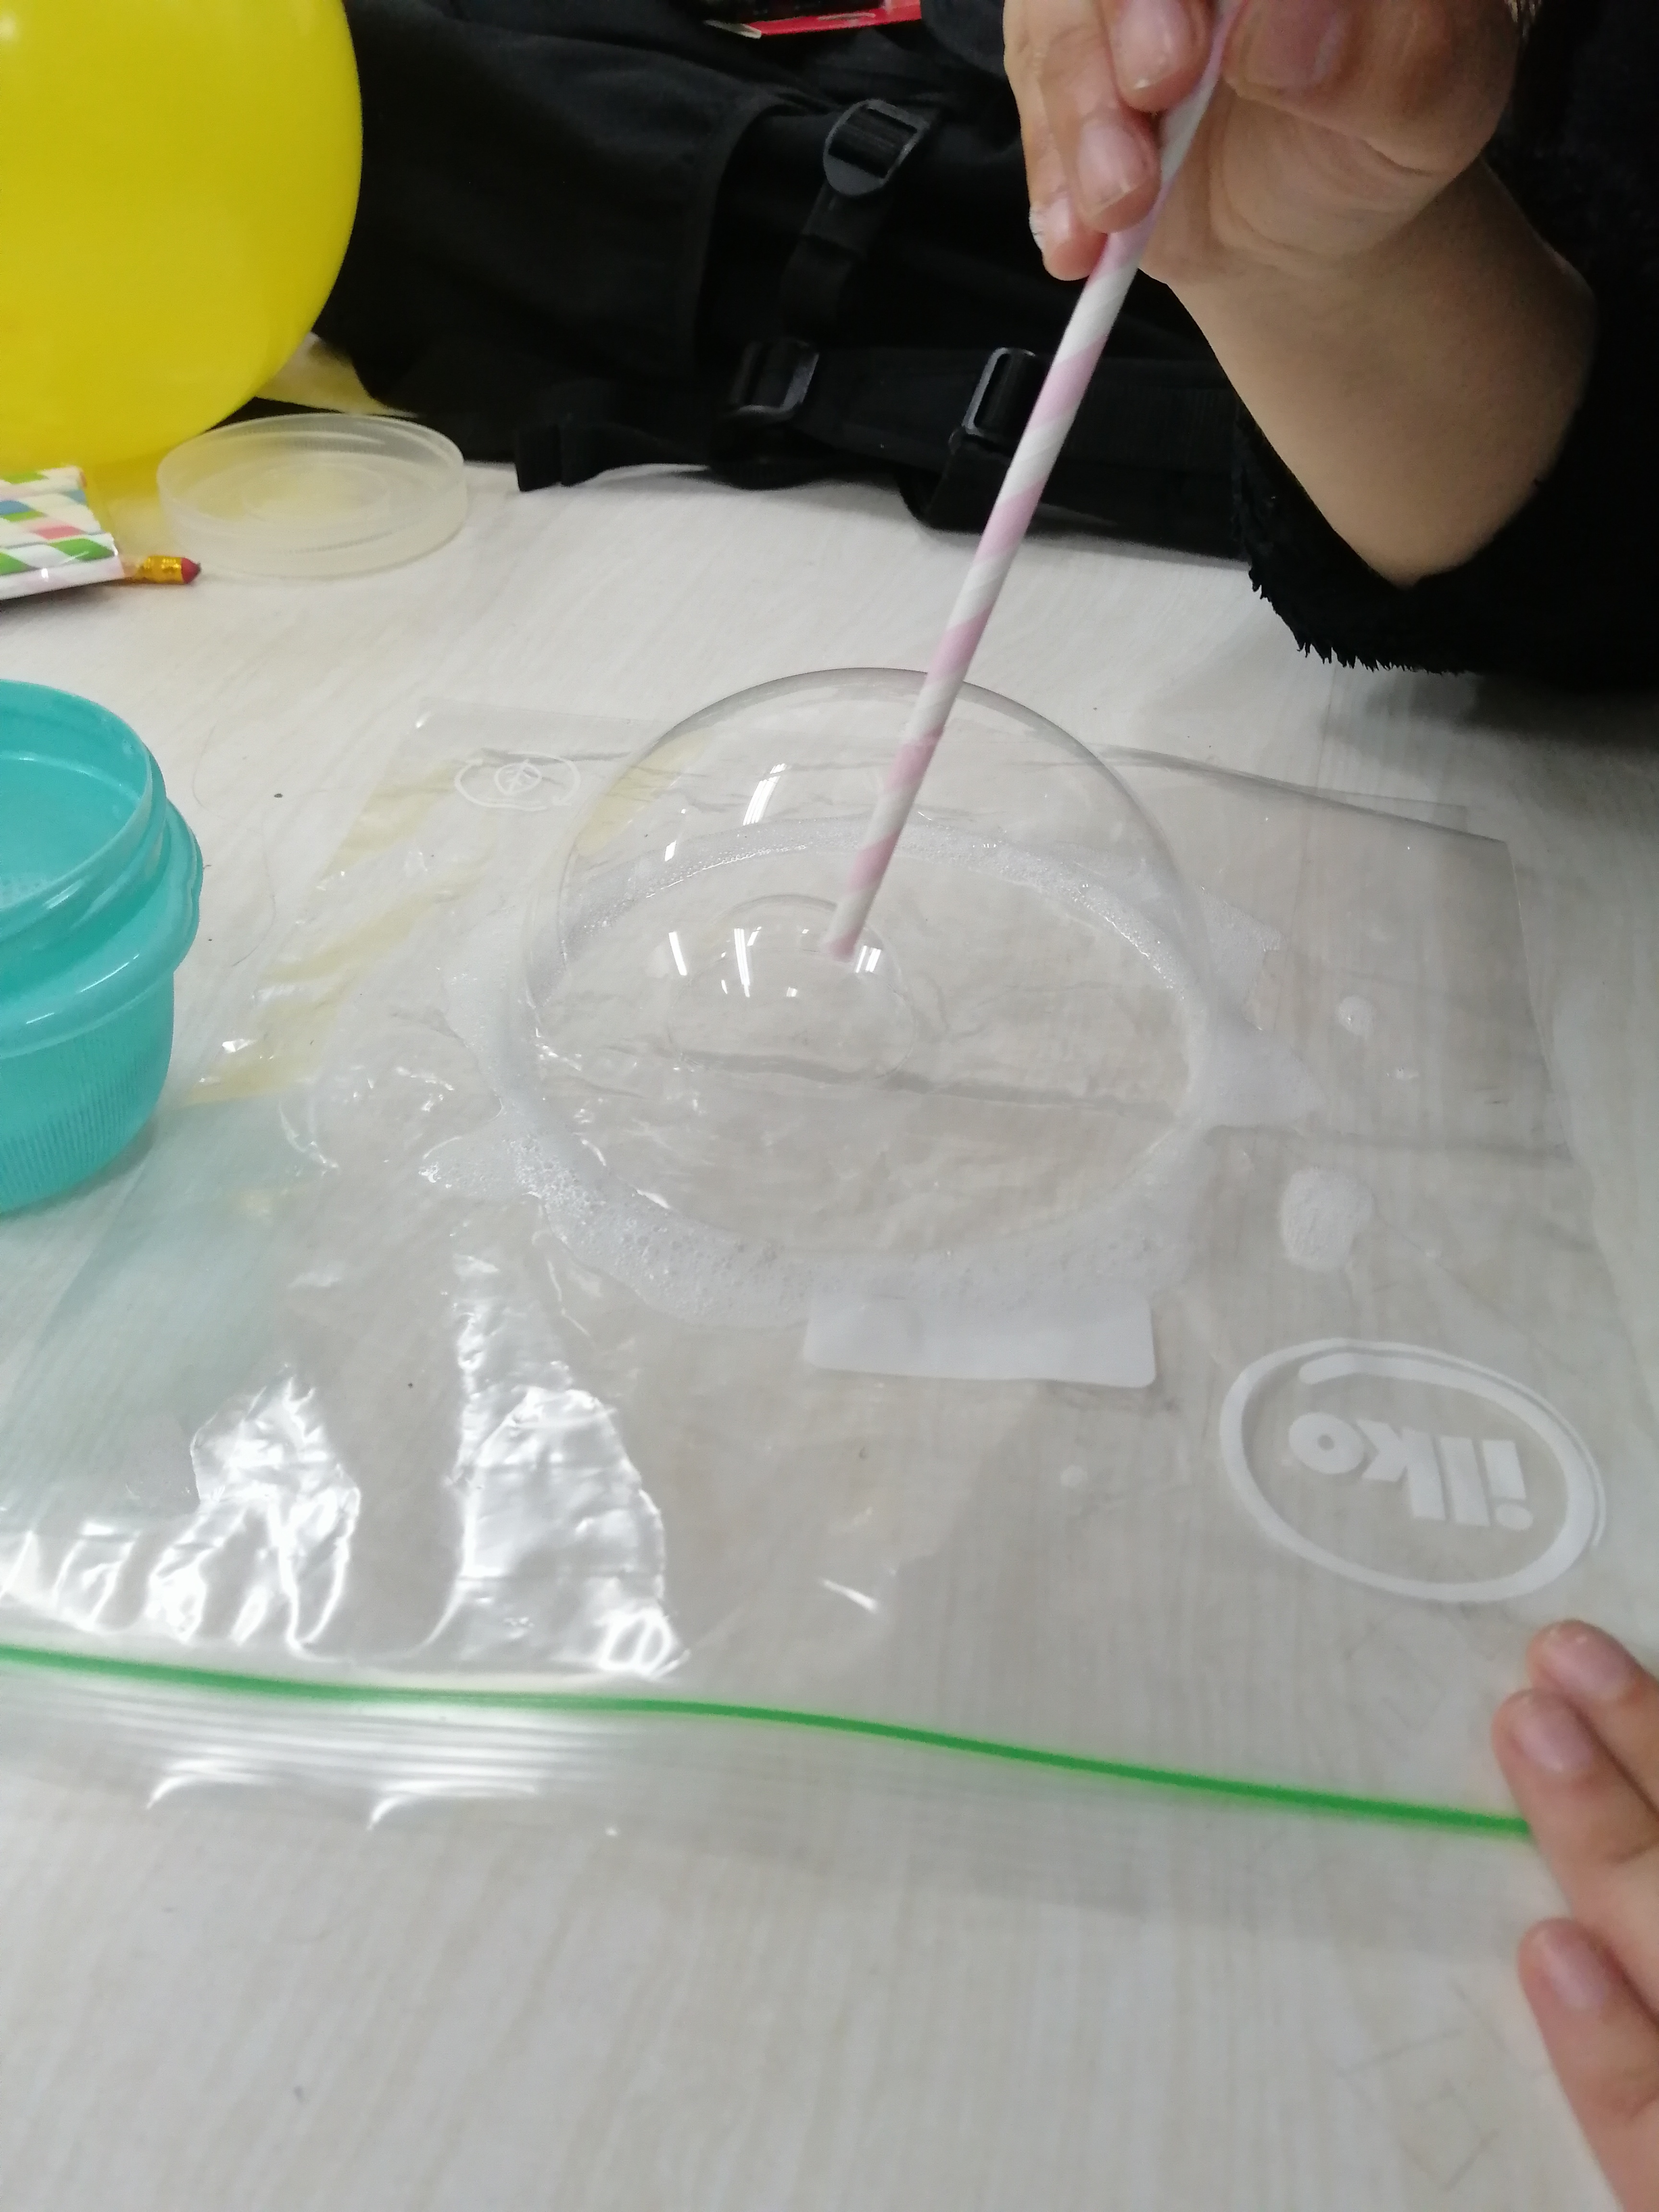
\includegraphics[width=4cm, height=5cm]{imag/Exp2_02.jpg}
    \end{subfigure}
\end{figure}


\begin{figure}[h!]
    \begin{subfigure}
        \raggedright
        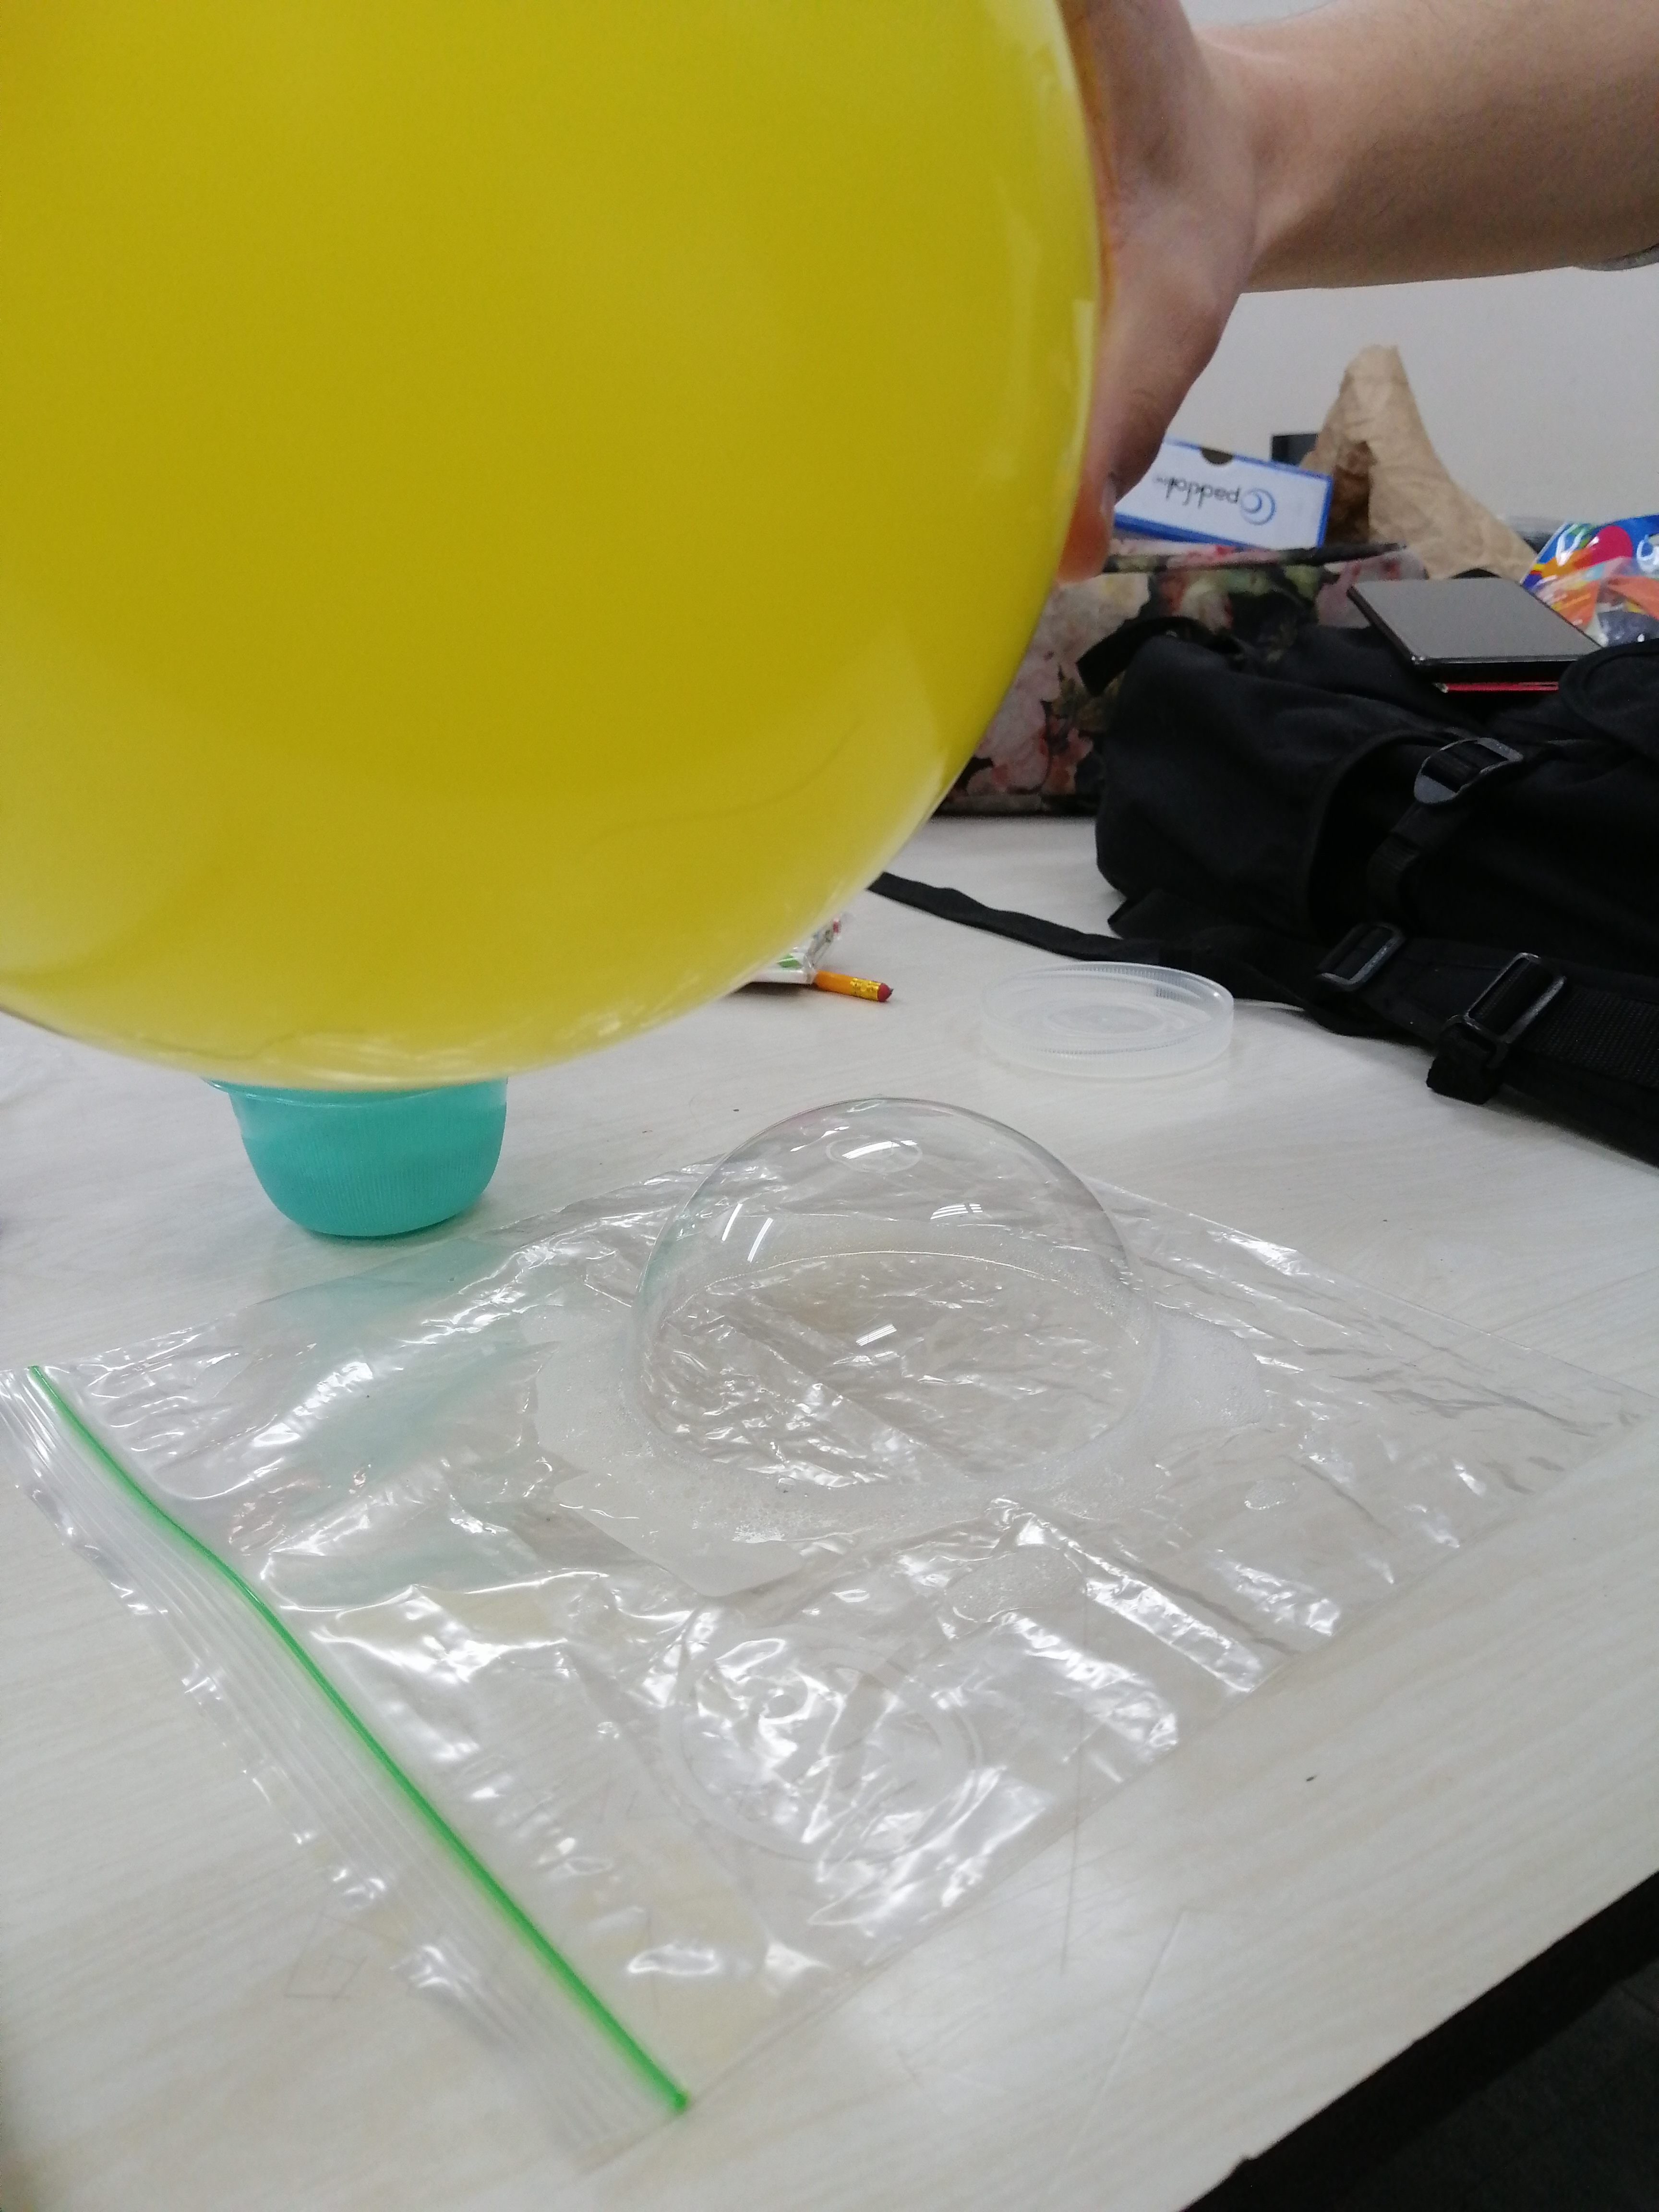
\includegraphics[width=4cm, height=5cm]{imag/Exp2_03.jpg}
    \end{subfigure}
    \begin{subfigure}
        \centering
        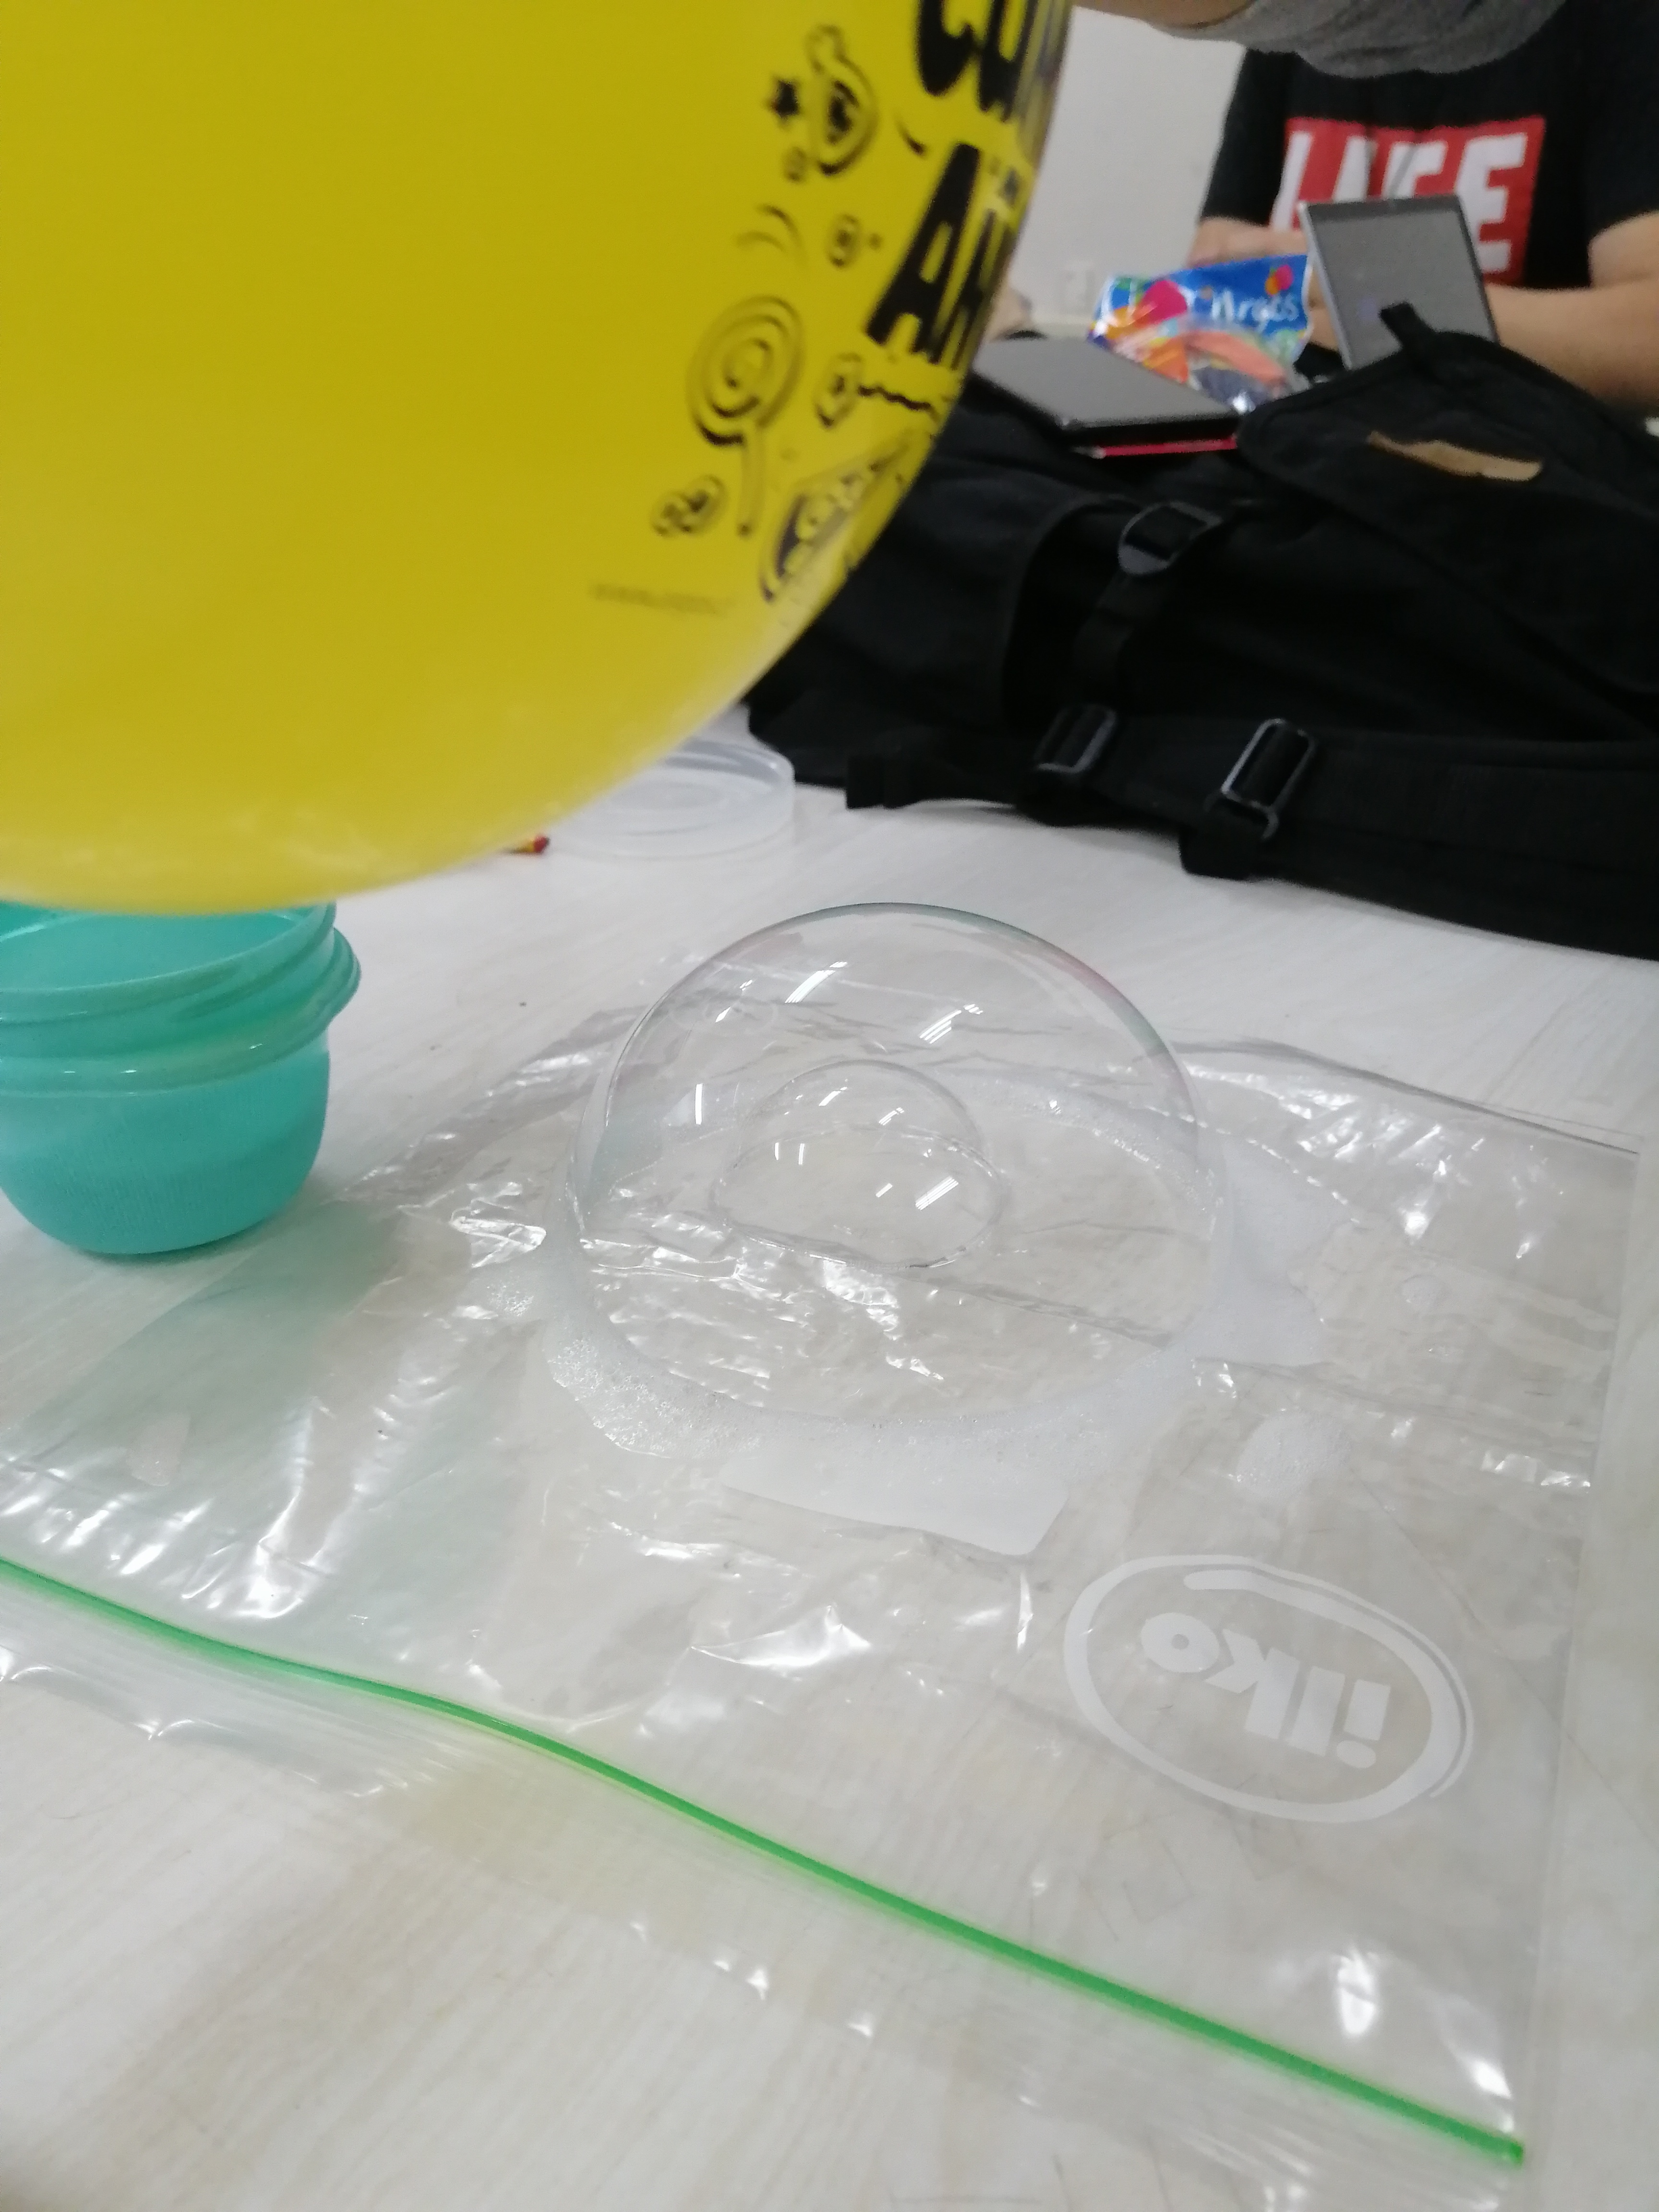
\includegraphics[width=4cm, height=5cm]{imag/Exp2_04.jpg}
    \end{subfigure}
\end{figure}
%%%%%%%%%%%%%%%%%%%%%%%%%%%%%%%%%%%%%%%%%%%%%%%%%%%%%%%%%%%%%%%%%%%%%%%
\newpage
\section*{Experimento 3}
\textit{Materiales: Colador de metal, celular, audífonos, papel de aluminio.}
    \begin{itemize}
        \item Encendermos la radio del celular.
        \item Luego, ponemos el móvil sobre el papel de aluminio.
        \item Finalmente, con el colador de metal, encerramos el área en donde se encuentra el celular.
    \end{itemize}

%imagenes%
\begin{figure}[h!]
    \begin{subfigure}
        \raggedright
        \includegraphics[width=4cm, height=5cm]{imag/Exp3_00.jpg}
    \end{subfigure}
    \begin{subfigure}
        \centering
        \includegraphics[width=4cm, height=5cm]{imag/Exp3_01.jpg}
    \end{subfigure}
\end{figure}

%============Análisis
\section*{Análisis}
Al ver detenidamente cada uno de los experimentos, podemos decir que guardan relación entre ellos.
En el primer experimento podemos notar que, cuando el teléfono lo envolvemos en papel de aluminio este no puede recibir llamadas ni tienen red wi-fi, esto nos quiere decir que el papel aluminio impide el paso de esas ondas electromagnetismo.
En el segundo experimento podemos ver que al acercar el globo cargado de electricidad a la burbuja pequeña que está en su interior.
En el tercer experimento podemos ver que al encerrar el teléfono con la radio puesta por abajo con el aluminio y por arriba con el colador de metal, la radio sufría interferencia, por lo que la antena que formaba los audífonos conectados al celular no recivbia señales de radio, de esto podemos decir que el papel aluminio con el colador de metal provocaban una barrera que abstruian el paso de ondas de electromagnéticas, en este caso las de radio.


%============Conclusión
\section*{Conclusión}
De lo anteriormente analizado en los 3 experimentos podemos ver que en todos se impedía el paso del campo eléctrico hacia el material que estaba dentro, esto es porque esos objetos como la burbuja grande , el aluminio y el colador de metal son conductores que en presencia de un campo eléctrico alcanzan el equilibrio electroestático en la que ya no hay movimientos de cargas, porque, el campo interno del conductor se opone al campo externo aplicado sobre el, de modo que en el interior del conductor el campo se vuelve nulo.
La ley de Gauss explica este fenómeno, yaqué reacciona el flujo de campo eléctrico a través de cualquier superficie cerrada es igual a la carga $q$ que está encerrada dentro de la superficie, dividida por la constante de la permitividad en el vacío $ε 0$, por lo que al no haber carga dentro del conductor, el campo eléctrico dentro de el es nulo, lo que explica porque la burbuja pequeña y el celular no percibía las ondas electromagnéticas y eléctricas.
Con este gran descubrimiento se pudieron crear objetos capaces de apantallar las ondas electromagnéticas y volverlas más seguras ante cualquier campo demasiado intenso para nosotros los humanos , como la famosa jaula de Faraday , la cual logra evitar los daños hacia los pasajeros de un avión cuando un rayo cae sobre ellos.

%============Referencias (en APA)












































\end{document}